\section{Introduction}

Only a few years ago, data centers were built around the compute space, vast data halls of servers, with power and cooling systems taking up a smaller share of the footprint. Then came the GPU revolution, transforming the data center into ``AI Factories''. As shown in Figure~\ref{fig:power-generation}, GPU racks are approaching 100 times greater power density compared to web servers and are increasing in power at a near-exponential pace, flipping the balance. Power infrastructure, once secondary, now rivals or even exceeds the space dedicated to compute.

\begin{figure}[h]
\centering
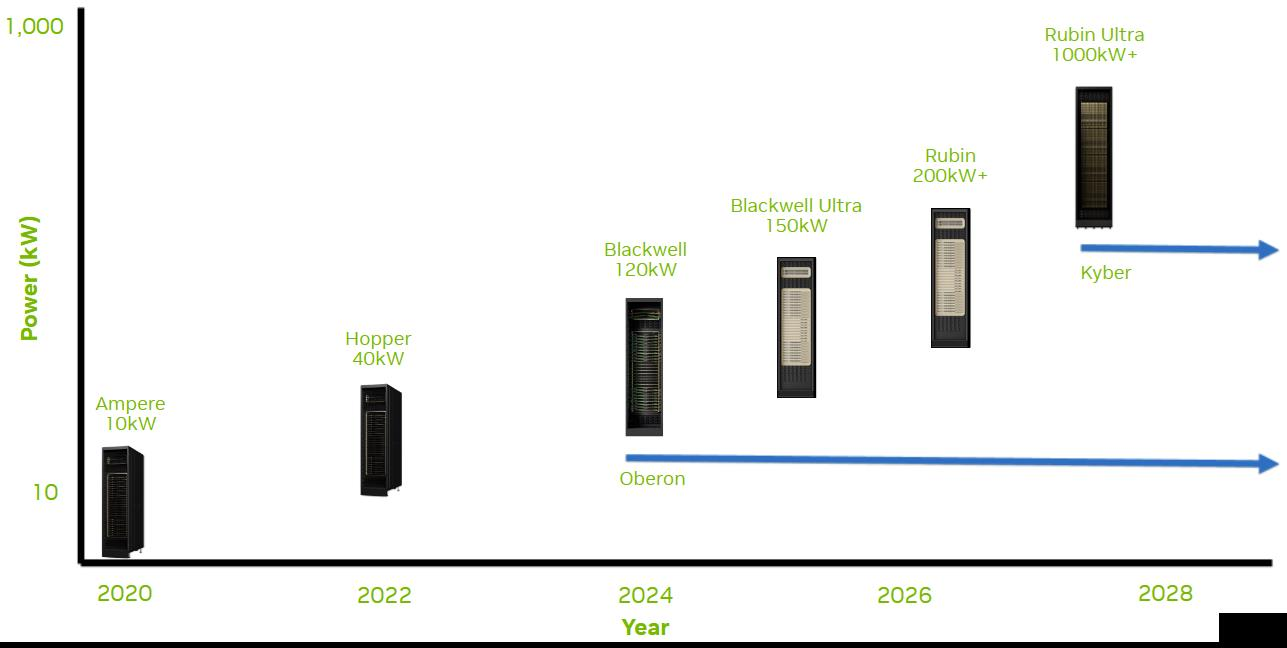
\includegraphics[width=0.8\textwidth]{figures/figure_p3_i1.jpeg}
\caption{Increasing Power Generation over Generation}
\label{fig:power-generation}
\end{figure}

As CPUs or GPUs are improved, there is typically an incremental increase in the GPU thermal design point (TDP) for power of 20\% generation over generation. This leads to an increase in power required per server over time. Nvidia's NVLink allows multiple GPUs to be networked together to effectively act as one large synchronous GPU and provide a significant improvement in performance when compared to operating over Ethernet connections. This networking of GPUs is most effective when connected over copper from both a power and cost standpoint, but at the expense of a limited reach due to signal integrity. Since the highest performance can be achieved when more GPUs are on the same copper domain with a limited reach, the maximum performance is tied to maximum power density. This means power increases are no longer 20\% generation over generation, but can easily be 2x, 4x or 8x with the increase in NVLink networking domain size.

\begin{figure}[h]
\centering
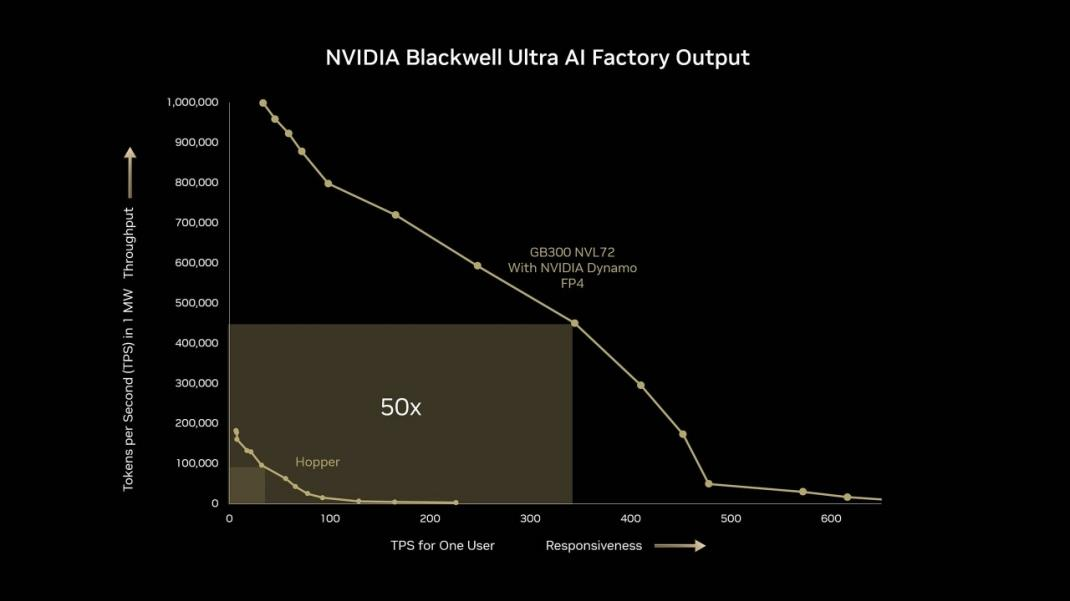
\includegraphics[width=0.8\textwidth]{figures/figure_p4_i1.jpeg}
\caption{A 75\% increase in TDP power, but a 50x increase in performance}
\label{fig:performance-increase}
\end{figure}

An example in Figure~\ref{fig:performance-increase} above is the performance increase from Hopper to GB300. The TDP power increased by 75\%, but the performance increased 50x with these changes. This also led to a 3.4x increase in rack power density going from an 4x8 GPU NVLink domains (32 in the rack) to a 72 GPU NVLink domain. As GPU packing and packaging improves and networking topologies move to larger domain sizes, this power density can continue to increase.

This increase in power generation over generation and with NVLink domain drives a much more rapid increase in power than has been seen in the past with GPUs. A secondary goal is to remove as many power components from the NVLink domain radius as possible since this is the highest value real estate in the rack for performance. This combination of driving to higher power level and pushing the power components away from the GPUs drives requirements for a different rack power architecture.

To meet these unprecedented demands, 800 VDC has emerged as the optimal architecture for next-generation power distribution. It allows for minimizing the conversion and routing volume in the compute space while minimizing datacenter distribution losses and total end to end conversion stages. 800 VDC significantly reduces current, copper use, and cable bulk compared to 54 VDC inside the rack or facility level 480 VAC systems, while remaining safe and scalable. It benefits from the growing maturity of Silicon Carbide (SiC) and Gallium Nitride (GaN) power conversion devices and the widespread adoption of 800 VDC systems in the electric vehicle (EV) industry. This enables seamless, end-to-end integration from grid to rack, higher power density beyond 1 MW.

Datacenters historically consisted of thousands of servers running diverse workloads. With GPUs these workloads can be synchronous across the datacenters leading to massive load swings in very short time intervals. Energy storage can be used to mitigate these swings. This rapid shift in datacenter power infrastructure requirements puts the industry at a crossroads. To keep up with future GPU demands, we need to rethink how we deliver power. This leads us to the next-generation distribution system that is more efficient, scalable, and ready for the extremely dynamic AI workloads. Integrating 800 VDC architectures with energy storage is key to future-proofing AI Factories for the era ahead.
